\chapter{Содержательная постановка задачи}

\section{Описание рабты существующей системы}

С точки зрания архитектуры программного продукта Информатикс делится на следующие части:

\begin{itemize}
    \item Moodle -- в качестве основного web-интерфейса сайта;
    \item Ejudge -- в качестве тестирующей системы;
    \item различные самописные модули на PHP, например, для управления группами учеников и для отрисовки наборов задач (далее по тексту -- конестов);
    \item различные самописные модули и API на Python, предоставляющие доступ к протоколам тестирования, сдачи кода пользователей и другое.
    \item СУБД MySQL 5.5.
\end{itemize}

Рассмотрим каждую часть подробнее.

\subsection{Ejudge}

Ejudge -- система для проведения различных мероприятий, в которых необходима автоматическая проверка программ. 
Она была разработана Алекстандром Черновым, предподавателем МГУ, в 2004 году. 
Система активно доробатывается и на текущий момент имеет более 11 тысяч коммитов в официальном репозитории.
Помимо этого, существует много различных дополнений системы, таких, как, например, 
патч к ядру Linux для более безопасного исполнения кода, ограничивающий доступ программы к некоторым возможностям операционной системы,
или файловая система, построенная на технологии FUSE, предоставляющая интерфейс сдачи задач в виде копирования файла с исходников в определенную примонтированную директорию.

Ejudge поддерживает следующие возиожности:

\begin{itemize}
    \item Проведение турниров с автоматической проверкой задач по четырём системам: ACM, KIROV, OLYMPIAD, MOSCOW.
    \item Ограниченные и неограниченные по времени турниры.
    \item Поддержка виртуальных турниров.
    \item Одновременное проведение нескольких турниров.
    \item Автоматическая регистрация участников турнира. Модерируемая регистрация участников турнира.
    \item Возможность участия в нескольких турнирах под одним регистрационным именем.
    \item Разделение прав доступа к турнирам. Некоторый пользователь может быть администратором одного турнира и не иметь никаких привилегий в другом турнире.
    \item Многоязыковой интерфейс. Текущая версия поддерживает русский и английский языки.
    \item Защищённое исполнение программ (если установлен патч к ядру).
    \item Поддержка вариантных задач, когда под одним именем каждый участник получает свой вариант задачи.
    \item Веб-интерфейс администратора и участника турнира.
    \item Веб-интерфейс администратора турнира для создания новых турниров и редактирования настроек существующих турниров.
    \item Настраиваемый внешний вид.
    \item Экспорт журнала турнира в формате XML.
    \item Экспорт внутренних таблиц (участников, журнала турнира, результатов) в формате CSV (comma-separated values).
    \item Доступ к серверам турниров из командной строки (возможность написания скриптов для управления турнирами).

\end{itemize}

Информатикс пользуется системой Ejudge в качестве тестирующей системы для кода пользователей (далее -- посылок).

В рамках проекта Информатикс Ejudge разделён на части -- Мастер-ejudge, который занимается непостредсвенно рагистрацией отправленных посылок, и Инвокеры (от англ. -- invoker, вызывающий), выполняющие прогон тестов для этих посылок. 

Ejudge -- действительно сложная система, исходный код содержит более 300 тысяч строк на языке C; 
для функционирования Ejudge даже был разработан собственный язык html-шаблонов, файлы с расширением csp, C-подобном языке,
который позволяют отрисовывать html-страницы с заданными параметрами. 

Ejudge работает с применением СУБД, в рамках проекта Информатикс -- СУБД MySQL 5.5.

\subsection{Moodle}

Moodle — система управления курсами (электронное обучение), также известная как система управления обучением или виртуальная обучающая среда. Является аббревиатурой от англ. Modular Object-Oriented Dynamic Learning Environment (модульная объектно-ориентированная динамическая обучающая среда). Представляет собой свободное (распространяющееся по лицензии GNU GPL) веб-приложение, предоставляющее возможность создавать сайты для онлайн-обучения.

Система Moodle используется в рамках проекта Информатикс в качестве основного Web-интерфейса платформы, 
курсы на Информатикс также реализованы с помощью Moolde.

На текущий момент в Информатикс используется устаревшая версия Moodle -- 1.8.2, вышедшая в 2012 году, при том, что актуальной является версия 3.6.3.

В Информатикс Moodle запущен под web-сервером apache HTTP Server (далее -- apache).

\subsection{Самописные модули и API на Python}

Часть запросов, отправляемых из web-интерфейса Informatics обрабатываются с помощью API (далее по тексту -- py-ручки, от англ. handlers) на Python, с использованием web-фреймворка Pyramid.
В качестве фреймворка для обращения к СУБД используется фреймворк SQLAlchemy.
Python-код запущен под uWSGI (веб-сервер и сервер веб-приложений, первоначально реализованный для запуска приложений Python через протокол WSGI). В то же время, uWSGI запущен под apache.
Запросы к Pyramid отделяются от остальных запросов по маске URI /py/ и с помощью проксирующего web-сервера nginx проксируются в apache.

Модули предоставляют следующий функционал:
\begin{itemize}
    \item отправка посылки на тестирование;
    \item отправка посылки на перетестирование;
    \item список посылок пользователя по задаче, списки посылок по пользователям и списки посылок по задачам;
    \item получение различной дополнительной информации по задачам -- например, примеры входных и выходных данных и др.
    \item рейтинг пользователей по количеству решённых задач;
\end{itemize}

и другое.

\section{Проблемы существующей системы}

\subsection{Выявленные проблемы пользователей при работае с Информатикс}

Основная жалоба пользователей на Информатикс -- постоянные сообщения об ошибке отправки задачи:
при сколько-нибудь значительном мероприятии, проводимом на Информатикс (например, одновременно 100 учеников), система перестаёт стабильно принимать посылки и отклоняет их с ошибкой\cite{inf_not_working}. 
Это мешало как простым пользователям-ученикам 
(кейс ученик на уроке информатики в школе пытается сдать задачу, и, хоть он её решил, у него не получается этого сделать), 
так и пользователям, участующем в мероприятии, так как обычно такие мероприятия имеют ограничения во времени.

С точки зрения создателей курса и пользователей LMS (далее -- учителей),
у сайта были проблемы с отображением результатов тестирования (далее -- мониторов).

Мониторы -- отображение количества решённых учеником задач в различных контестах, собранное в единую таблицу.

Мониторы работали очень медленно, а если количество результатов было достаточно большим 
(например, более 50 задач в контесте и более сотни учеников), 
не работали вообще (как было выяснено позднее, они специально были отключены патчем, так как сильно нагружали систему).

Помимо этого, были зафиксированы абстрактные жалобы на то, что сайт часто работает медленно -- <<тормозит>>. 
Особенно сильно это заметно по воскресеньям, когда Информатиксом практически невозможно пользоваться.

\subsection{Описание архитектурных проблем системы}

В Информатиксе было выявлено множество различных архитектурных проблем и недочётов, 
которые с повышением нагрузки на ресурс, начали давать о себе знать.

Самая большая сложность Информатикс -- в системе тестирования Ejudge, которая имеет корневые недостатки, неисправимые в текущих реалиях, например:
\begin{itemize}
    \item Общение Мастер-Ejudge и Инвокеров происходит через через файловую систему\cite{ejudge_jobs}. 
    В ФС сохраняются так же и исходные коды посылок, и результаты их тестирования.
    \item Посылка не имеет единственного уникального идентификатора в базе данных; она идентифицируется в рамках объединённого ключа, состоящего из номера посылки в рамках контеста и идентификатора контеста.
    \item Система Ejudge -- синхронна и не может предварительно сохранить посылку перед непосредственной обработкой.
    \item Код Ejudge сложен для понимания и плохо документирован\cite{ejudge_source}.
\end{itemize}

Общение через файловую систему и хранения в ней исходных кодов посылок, результатов и протоколов тестирования даёт нам следующие проблемы:

\begin{itemize}
    \item За годы работы на файловой системе накопилось более полутерабайта файлов.
Этих файлов -- десятки миллионов, при том, что размер конкретного файла часто не превышает нескольких байт.
    \item При необходимости сделать бэкап, нужно скопировать каждый файл, лежащий на ФС, что даёт огромную нагрузку на ресурс диска
(более 99\% операций ввода-вывода в секунду (англ. Input-Output operations per second -- IOPS) в это время приходится на бэкап). 
Бэкапы заланированы каждую неделю в воскресенье, что и даёт практически полую недоступность ресурса в это время.
    \item Инвокеры могут быть запущены на отличных от Master-ejudge машинах, что позволяет удобно масштабировать (далее -- скалировать) их (например, есть задачи, тестирование посылок которых занимает более 15 минут). 
    Однако им приходится всё так же поддерживать связь между собой и Master-ejudge через ФС, 
    что было достигнуто использованием SSHFS (Secure SHell FileSystem -- клиентская программа, работающая через модуль FUSE и используемая для удаленного управления файлами по протоколу SSH (точнее, его расширению SFTP) таким образом, как будто они находятся на локальном компьютере).
    Это даёт нам необходимость очень широкого и быстрого канала Ethernet-соединения, что в текущих реалиях может быть достигуто только с помощью разворачивания Инвокеров на одной и той же хост-машине, что и Master-ejudge.

\end{itemize}{}


Отсуствие уникального идентификатора посылки даёт нам следующие проблемы:

\begin{itemize}
    \item Ejudge плохо масштабируется, потому что, так как у посылки нет уникального идентификатора, 
нет возможности сделать несколько независимых друг от друга систем Ejudge так, чтобы они работали через одну СУБД.
    \item Запросы в СУБД, необходимые для построения мониторов -- сложные, долго обрабатываются и сильно нагружают СУБД.

Синхронность Ejudge даёт нам следующие проблемы:

    \item Master-Ejudge синхронно обрабатывает отправленные посылки, что означает, что 
если какая-то посылка обрабатывалась долго, другие посылки оправить не получится
(появится сообщение <<Ошибка отправки задачи>>).
    \item Проблема из предыдущего пункта заставляет пользователей постоянно повторно отправлять посылки, что ещё больше нагружает систему.
\end{itemize}

Сложность и плохая документированность кода Ejudge даёт нам следующие проблемы:
\begin{itemize}
    \item Невозможность за какие-либо разумные сроки исправить архитектурные проблемы Ejudge, представленные выше.
\end{itemize}

Помимо этого есть общие проблемы, связанные с использованием Ejudge в информатикс -- например, 
хотелось бы иметь возможность использовать кэширование результатов мониторов, что позволило бы уменьшить нагрузку на СУБД;
однако такой кэш должен инвалидироваться -- <<протухать>> -- при изменении результатов (например, при отправке новой посылки).

Однако это реализовать такую систему кэша не представляется возможным, 
так как Ejudge не даёт нам возможность каким либо образом узнать, что посылка протестировалась, 
кроме как постоянным сканированием БД, что даёт нам большую нагрузку
или подпиской на обновления ФС, например, с помощью подсистемы ядра Linux Inotify), \label{chap:inotify}
что невозможно, так как в ФС хранятся десятки миллионов файлов\cite{many_files}.

В рамках текущей архитектуры в одной СУБД MySQL были использованы следующие БД:
\begin{itemize}
    \item moodle -- БД, используемая преимущественно системой Moodle в которой хранятся пользователи, курсы и наборы задач;
    \item ejudge -- БД, используемая преимущественно для нужд системы Ejudge, в ней хранятся посылки пользователей и настройки задач;
    \item pynformatics -- БД, используемая преимущественно py-ручками.
\end{itemize}
Была активно использована особенность СУБД MySQL -- базы данных в ней представляются одновременно и схемами БД, 
что даёт возможность построения SQL-запросов, использующих данные одновременно нескольких БД.

% TODO: схема разбивки VM-ки
% TODO: написать про 15кк посылок

Это выливается в потерю производительности и невозможность разделить СУБД MySQL на несколько инстансов, 
которые можно было бы развернуть на раздельных машинах.

\begin{figure}
  \centering
  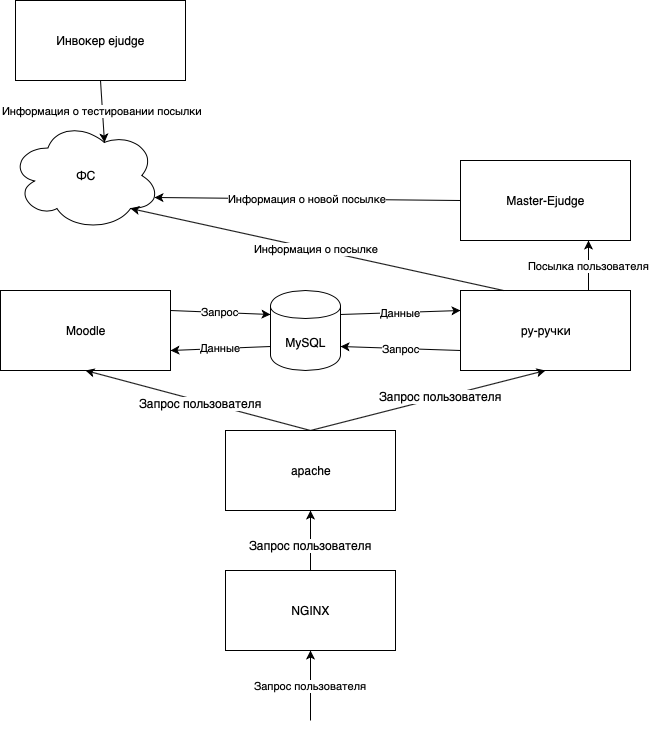
\includegraphics[width=\textwidth]{figures/old_informatics.png}
  \caption{Схема работы Информатикс}
  \label{fig:old_informatics}
\end{figure}

\section{Постановка задачи}

Для решения указанных выше проблем необходимо разработать и улучшить архитектуру, чтобы:

\begin{itemize}
    \item Уменьшить нагрузку на ФС, которой сложно предоставлять доступ к большому количеству файлов.
    \item Добавить возможность встраивать несколько различных тестирующих систем, включая тестирующие системы отличные от Ejudge.
    \item Исправить и ускорить сбор данных для мониторов.
    \item Сократить или полностью избавиться от необходимости использования SQL-запросов, обращающихся к разным БД.
    \item Улучшить общую производительность системы.
    \item Улучшить взаимодействия пользователей с системой 
    -- сделать так, чтобы ошибка отправки решений пропала,
    а посылки принимались сразу и последовательно тестировались.
\end{itemize}

Также необходимо разработать и реализовать архитектурный задел для дальнейшего развития Информатикс в качестве базы задач для встраивания в другие системы.

Помимо этого, нужно разарботать и реализовать план изменения архитектуры системы таким образом, чтобы недоступность системы была минимальной.